\documentclass[11pt]{article}

\usepackage[utf8]{inputenc}


\usepackage[a4paper,margin=1in]{geometry}
\usepackage{amsmath,amssymb,amsthm}
\usepackage{graphicx}
\usepackage{booktabs}
\usepackage{array}
\newcolumntype{L}[1]{>{\raggedright\arraybackslash}p{#1}}
\usepackage{enumitem}
\usepackage[font=small,labelfont=bf]{caption}
\usepackage{subcaption}
\usepackage{xcolor}
\usepackage[colorlinks=true,linkcolor=blue!60!black,citecolor=blue!60!black,urlcolor=blue!60!black]{hyperref}
\usepackage{microtype}

\setlist{itemsep=2pt,topsep=4pt}
\newtheorem{proposition}{Proposition}
\newcommand{\norm}[1]{\lvert #1\rvert}
\newcommand{\Vsub}{2\text{k}}
\newcommand{\rev}[1]{#1}

\title{Can a sparse autoencoder find the token embeddings?\\[2pt]
\large A toy model of SAE training with a known answer}
\author{Navid Nabijou\thanks{Queen Mary University of London. \texttt{nn333@cantab.ac.uk}}}
\date{October 30, 2026}

\begin{document}
\maketitle

\begin{abstract}
Sparse autoencoders (SAEs) are trained to find interpretable features in neural networks, but the true features are unknown, so a failure is hard to diagnose. We study a setting where the answer is known. The data are the rows of GPT-2 Small's token embedding table, and the SAE has exactly one feature per token. With no bottleneck, the natural target is the embedding table itself: one feature along each token's embedding. We train from random initialisation and measure how much of the target training recovers. Both common SAE architectures can recover it, but they need very different regimes. A ReLU SAE with an L1 penalty recovers 93\% of the full table, and up to 98\% of a 2,000-token subvocabulary, across a wide region of hyperparameters. A penalty that is too strong kills features, and one that is too weak needs ever longer training; with no penalty at all, nothing is recovered. A TopK SAE fails with any fixed $k$, because a small $k$ kills features and a large $k$ spreads each token over several features. Lowering $k$ during training to 1 succeeds, but slowly: on the subvocabulary it reaches 89\% after eight times the training that gave ReLU 98\%, and it is still improving. For both architectures, recovery does not depend on the vocabulary size once training is scaled in proportion to it. A small subvocabulary is therefore a faithful model of the full problem, and the full-scale runs bear this out.
\end{abstract}

\section{Introduction}

A sparse autoencoder (SAE) rewrites each input vector as a sparse combination of learned directions, called features. SAEs have become a standard tool for finding interpretable features in the activations of language models \cite{cunningham2023sparse,bricken2023monosemanticity,templeton2024scaling,gao2024scaling}. The hope is that each feature corresponds to one concept the model uses.

Training an SAE is not easy. Two problems recur in the literature. The first is the trade-off between sparsity and reconstruction: a sparser code reconstructs the input less well. The second is \emph{dead features}: features that stop activating on any input during training, and so stop receiving gradient \cite{bricken2023monosemanticity,gao2024scaling}. Several remedies exist, and they are judged by how many features stay alive and how well the SAE reconstructs its input. A harder question is whether the resulting features are the right ones, because in real activations the true features are unknown. When an SAE fails to produce a clean feature, the cause could be the training, the size of the dictionary, or the absence of any such feature in the data.

\paragraph{A toy model with a known answer.} We study a setting where the answer is known. The data are the rows of the input embedding table of GPT-2 Small \cite{radford2019language}: $V = 50{,}257$ vectors in $d = 768$ dimensions, one per token. These are the \emph{raw} token embeddings: the vectors the model looks up for each token before any layer runs. Unlike contextual embeddings, they do not depend on the surrounding text. We give the SAE exactly as many features as there are tokens, $m = V$.

With $m = V$ there is no bottleneck. Every token can have a feature of its own. A one-hot code, in which each token is rebuilt by a single feature pointing along it, reconstructs every token exactly. It is also as sparse as a code can be. The natural target for the SAE is therefore the embedding table itself: one feature per token, along that token's embedding. Sections~\ref{sec:topk-target} and~\ref{sec:relu-target} make this precise for each architecture.

This makes $m = V$ a toy model of SAE training. Because the target is known, we can measure how much of it training finds: a token is \emph{recovered} if some feature matches its embedding. Because capacity is not the limit, any token that is not recovered is a failure of training. We train from random initialisation, as in practice, and ask which architectures and settings find the target, and at what cost. Figure~\ref{fig:headline} previews the answer on a 2,000-token subvocabulary.

\begin{figure}[t]
\centering
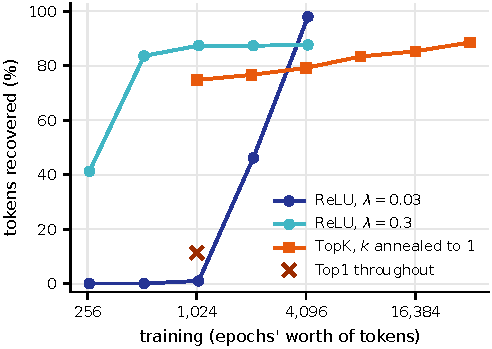
\includegraphics[width=0.58\linewidth]{figures/headline.pdf}
\caption{Share of tokens recovered against the amount of training, on the 2,000 most frequent tokens with $m = 2{,}000$. One epoch's worth is 2,000 training examples. Blue: ReLU SAEs with an L1 penalty $\lambda$ (Section~\ref{sec:relu}). Orange: TopK SAEs with $k$ lowered from 128 to 1 during training (Section~\ref{sec:topk}). Each orange point is a separate run of that length. The cross is a TopK SAE trained at $k = 1$ throughout.}
\label{fig:headline}
\end{figure}

\paragraph{Findings.} The findings fall into three themes.
\begin{enumerate}[leftmargin=*]
\item \textbf{TopK SAEs recover the embeddings only when $k$ is annealed to 1, and at a high training cost.} With a fixed $k$ they fail. A small $k$ leaves most features dead, and a large $k$ spreads each token over $k$ features. Starting at a large $k$ and lowering it to 1 works. Every drop in $k$ kills features, but the features that survive are almost all correct. More training saves more features. On the subvocabulary, recovery rises by about 3 percentage points per doubling of training, to 89\% at the longest run, with no sign of levelling off (Section~\ref{sec:topk}).
\item \textbf{ReLU SAEs with an L1 penalty recover the embeddings across a wide region of hyperparameters}: 98\% of the subvocabulary and 93\% of the full table. Outside that region they fail in one of two ways. With too little training, codes stay dense. With too much pressure, features die. The penalty must be weak but not zero: a weaker penalty recovers more but needs longer, and no penalty recovers nothing (Section~\ref{sec:relu}).
\item \textbf{With training scaled to the vocabulary, recovery does not depend on its size}, for both architectures. Subvocabularies of 2,000, 5,000, 10,000 and 20,000 tokens give the same recovery, to within a few points, when the number of training steps grows in proportion to $V$. A small subvocabulary is therefore a faithful model of the full table, and the full-scale runs agree with it (Section~\ref{sec:sizes}).
\end{enumerate}

Several of the ideas we use, and some of the effects we found, also appear in Gao et al.~\cite{gao2024scaling}. These include the TopK architecture, the trade-off between sparsity and dead features, the auxiliary loss we test in Section~\ref{sec:auxk}, the scaling of the learning rate with the number of features, and the growth of training cost with that number. We point out each overlap where it arises.

Section~\ref{sec:setting} describes the setting. Sections~\ref{sec:topk} to~\ref{sec:sizes} give the results for the three themes. Section~\ref{sec:discussion} offers labelled speculation, Section~\ref{sec:limitations} states the limitations and Section~\ref{sec:related} reviews related work. The appendices give the mathematical arguments, the training details and the full results.

\section{Setting and methods}
\label{sec:setting}

\subsection{Data}

The data are the rows $x_1, \dots, x_V \in \mathbb{R}^{768}$ of the GPT-2 Small input embedding table. Besides the full table, we use subvocabularies made of the $V$ most frequent tokens, for $V$ = 2,000, 5,000, 10,000 and 20,000. Frequency is counted on about 200 million tokens of English Wikipedia. It is used only to choose which tokens make up a subvocabulary. Training samples tokens uniformly at random, and evaluation weights every token equally. Most of our exploratory runs use the 2,000 most frequent tokens, which we call \emph{the 2k subset}.

\subsection{Two architectures}

Both SAEs reconstruct a token $x$ as
\begin{equation}
\hat{x} = \sum_{j=1}^{m} f_j(x)\, d_j ,
\end{equation}
where $d_j \in \mathbb{R}^{768}$ is the decoder row of feature $j$ and $f_j(x) \ge 0$ is its coefficient. Decoder rows have unit length and there is no decoder bias. The encoder computes pre-activations $a_j(x) = w_j \cdot x + b_j$.
\begin{itemize}[leftmargin=*]
\item \textbf{TopK} \cite{makhzani2013ksparse,gao2024scaling}. Only the $k$ largest pre-activations are kept, with a ReLU applied to them, and the others are set to zero. The loss is the squared error $\norm{x - \hat{x}}^2$. With $k = 1$ we call it \emph{Top1}.
\item \textbf{ReLU with an L1 penalty} \cite{bricken2023monosemanticity,cunningham2023sparse}. The coefficients are $f_j = \mathrm{ReLU}(a_j)$, and the loss is
\begin{equation}
L = \norm{x - \hat{x}}^2 + \lambda \sum_j f_j .
\end{equation}
\end{itemize}
Initialisation uses no information from the embeddings. The decoder rows are random Gaussian directions, the encoder weights start as the transpose of the decoder, and the encoder biases start at zero. After initialisation the encoder and decoder are trained as separate parameters. Initialising the encoder along the decoder directions follows Gao et al.~\cite{gao2024scaling}.

\subsection{Training}

We use Adam \cite{kingma2015adam} at a constant learning rate. Gao et al.~\cite{gao2024scaling} found that the largest stable learning rate for TopK SAEs scales as $1/\sqrt{m}$. We follow this scaling for both architectures and normalise it ourselves to
\begin{equation}
\eta_{\mathrm{Gao}} = 2 \times 10^{-4} \Big/ \sqrt{m / 2^{14}} ,
\end{equation}
which we call \emph{the Gao rate}. It is about $5.7\times10^{-4}$ on the 2k subset and $1.1\times10^{-4}$ on the full table. Each minibatch draws tokens uniformly at random, with replacement.

We measure the amount of training in two ways. An \emph{epoch's worth} is $V$ training examples, so a run of $S$ steps at batch size $B$ has $SB/V$ epochs' worth. \emph{Gao-rate steps} are steps multiplied by the learning rate as a multiple of the Gao rate. At a fixed vocabulary size, Gao-rate steps turn out to be what counts (Sections~\ref{sec:levers} and~\ref{sec:regimes}).

\subsection{Measurement}

A token is \emph{recovered} if some decoder row is its mutual nearest neighbour by cosine similarity, at a cosine above 0.9. We also report the stricter threshold of 0.99. A feature is \emph{alive} if it is active, with a positive coefficient, on at least one token. All measurements use every token of the vocabulary.

Most runs use one seed. Repeated runs on the 2k subset differ by about 40 tokens between seeds, and by about the same between machines. A single run is therefore good to about $\pm20$ tokens, or $\pm1$ percentage point, on the 2k subset. Appendix~\ref{app:setup} gives the full training setup of every run, and Appendix~\ref{app:results} gives the results as tables.

\section{TopK SAEs: recovery by annealing \texorpdfstring{$k$}{k}, at a high cost}
\label{sec:topk}

\subsection{The target}
\label{sec:topk-target}

A Top1 SAE rebuilds each token from one decoder row times a non-negative coefficient. The rows have unit length, so a token $x$ is rebuilt exactly if and only if some row equals $x/\norm{x}$. With $m = V$, the dictionary with zero loss is therefore the set of normalised embeddings. It is unique up to the order of the features, as long as no two embeddings point the same way.

For $k > 1$ this uniqueness is lost. A token can be rebuilt from several features, and many other dictionaries also reach zero loss. So only Top1 makes the embeddings the unique target.

\subsection{Sparsity against keeping features alive}
\label{sec:tradeoff}

A TopK feature receives gradient only on the tokens where it is among the top $k$. A feature that is never selected gets no gradient, so it does not move.\footnote{In principle a dead feature can still revive. It gets no gradient itself, but the features above it keep training, and they can move away from a token and leave it to the dead feature. In practice this never happened in our Top1 runs: on the full table, none of the 39,914 features dead at initialisation revived.} This creates a trade-off between sparsity and keeping features alive, which Gao et al.~\cite{gao2024scaling} also identify as a central difficulty.

\textbf{Top1 from the start fails.} On the full table, only 20.6\% of features are among the top 1 for some token at initialisation. Training a Top1 SAE did not revive a single one of the others. The alive features then collapsed from 10,343 to 259 within the first 5\% of training, and only 16 tokens were recovered. On the 2k subset the picture is similar: 382 features stay alive and 227 tokens are recovered (Figure~\ref{fig:headline}, cross).

\textbf{A larger fixed $k$ fails the other way} (Figure~\ref{fig:topk-k}a). Raising $k$ keeps more features alive: 89\% at $k = 32$, against 19\% at $k = 1$. But every token then uses all $k$ slots. The dictionary of normalised embeddings still has zero loss, but it is no longer the only one: many other dictionaries rebuild every token exactly from several features. The loss is indifferent between them, so nothing pulls each feature onto a single token. Recovery falls as $k$ rises, and is gone by $k = 16$.

\begin{figure}[t]
\centering
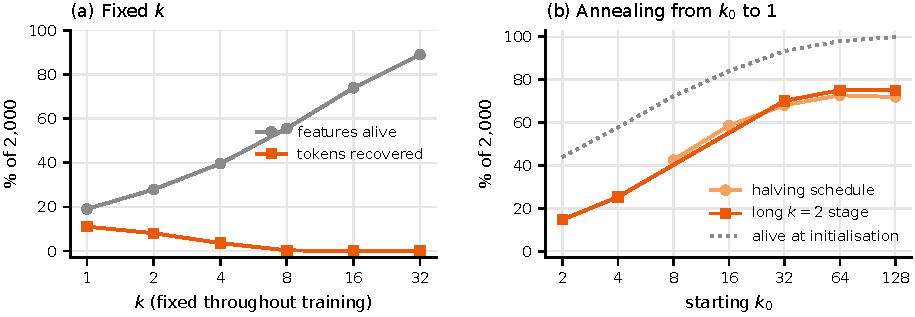
\includegraphics[width=\linewidth]{figures/topk_k.pdf}
\caption{TopK SAEs on the 2k subset. (a) Fixed $k$ throughout training (3,000 steps). A larger $k$ keeps more features alive but recovers fewer tokens. (b) $k$ lowered from $k_0$ to 1 during training (4,000 steps). Two schedule shapes (Section~\ref{sec:anneal}). The dotted line is the share of features alive at initialisation for $k = k_0$. Recovery rises with $k_0$ until nearly all features start alive.}
\label{fig:topk-k}
\end{figure}

\subsection{Annealing: features die only at the drops, and the survivors are correct}
\label{sec:anneal}

\emph{$k$-annealing} tries to have both. Training starts with a large $k$, so that features stay alive and spread out over the embeddings. $k$ is then lowered in stages until it reaches 1, so that each token is pushed onto a single feature. Our main schedule halves $k$ from $k_0$ down to 4 in equal stages over the first 40\% of training. It then holds $k = 2$ for 40\% and $k = 1$ for the last 20\%. We call this the schedule with a long $k = 2$ stage. Figure~\ref{fig:topk-k}b also shows a plain halving schedule, which reaches $k = 1$ at 80\% of training.

Annealing works (Figure~\ref{fig:topk-k}b). From $k_0 = 64$ or 128, it recovers 75\% of the 2k subset in 4,000 steps, against 11\% for Top1 throughout. Figure~\ref{fig:anneal} shows how. It follows a run with $k_0 = 128$ through training. Three facts stand out.
\begin{itemize}[leftmargin=*]
\item \textbf{Features die only at the drops in $k$.} Between drops the alive count is flat. Most deaths happen at the final drop, from $k = 2$ to $k = 1$, which costs about 20\% of the alive features in this run. A large $k_0$ also revives the features that start dead: at full scale, $k_0 = 128$ revived all 3,349 of them early in training.
\item \textbf{Features which die at a drop almost never revive.} Once a feature has died at a drop, it stays dead.
\item \textbf{The survivors are correct.} At the end, 1,495 tokens are recovered by 1,515 alive features. Across all our annealed runs, 96\% to 100\% of the surviving features are recovered tokens. This is the opposite of Top1 from the start, where most survivors match no token. So recovery after annealing is essentially the number of features that survive.
\end{itemize}

\begin{figure}[t]
\centering
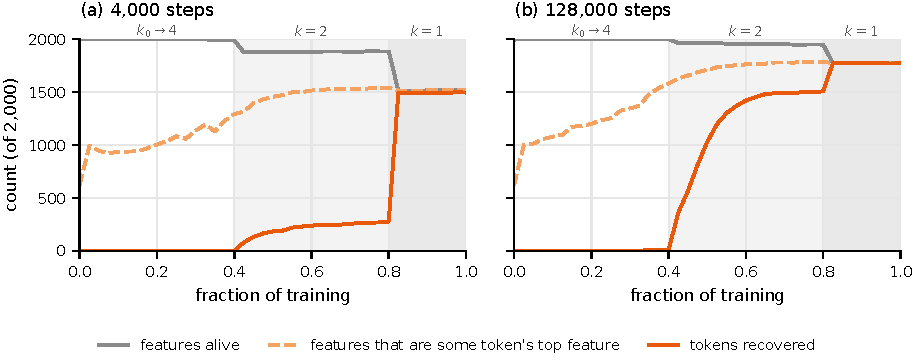
\includegraphics[width=\linewidth]{figures/anneal_dynamics.pdf}
\caption{One annealed TopK run on the 2k subset, $k_0 = 128$ with a long $k = 2$ stage. The shading marks the $k = 2$ and $k = 1$ stages. Grey: alive features. Dashed: features that are the top feature, with a positive pre-activation, of at least one token. Orange: recovered tokens. At the drop to $k = 1$, the alive count falls to the dashed line. (a) 4,000 steps. (b) 128,000 steps: more features are some token's top feature when $k$ drops to 1.}
\label{fig:anneal}
\end{figure}

Which features survive the final drop? At $k = 1$ a feature is active only on tokens for which it is the top feature. So a feature survives the drop only if it is the top feature of at least one token at that moment. The dashed line in Figure~\ref{fig:anneal} counts these features. The alive count falls exactly onto it at the drop: across all our runs this count predicts the survivors to within about 2\%. The final drop is therefore a competition for a limited number of slots. A feature that comes second for every token it serves dies at once.

\subsection{An auxiliary loss cannot rescue the dead features}
\label{sec:auxk}

Gao et al.~\cite{gao2024scaling} revive dead features with an auxiliary loss, AuxK. It trains the dead features to reconstruct the residual $x - \hat{x}$ that the live features leave behind. In their setting it removes nearly all dead features. In ours it does not help. Adding AuxK to the run of Figure~\ref{fig:anneal}a gave 1,476 and 1,478 recovered tokens at two loss weights, against 1,499 for the same run without it. A variant that trains the dead features on the whole token at $k = 1$ gave at most about 40 tokens more, which is within the noise.

The reason is that the problem is competition, not a lack of gradient. Suppose a live feature codes a token $x$ at an angle $\theta$, and a dead feature lines up with the residual. The residual is perpendicular to the live feature, so the dead feature's pre-activation on $x$ is about $\norm{x}\sin\theta$, while the live feature's is about $\norm{x}\cos\theta$. At a cosine of 0.9, that is $0.44\norm{x}$ against $0.9\norm{x}$. The dead feature trains, but it never wins the token. Appendix~\ref{app:auxk} gives the details.

\subsection{Two levers: the starting \texorpdfstring{$k$}{k} and the amount of training}
\label{sec:levers}

\textbf{The starting $k$.} Recovery rises with $k_0$ until nearly every feature is alive at initialisation, and then levels off (Figure~\ref{fig:topk-k}b). On the 2k subset this happens at $k_0 = 64$, where 98\% of features start alive. The shape of the schedule matters much less. Moving time between the low stages, or adding a stage at $k = 3$, changes recovery by at most about 40 tokens.

\textbf{The amount of training.} Figure~\ref{fig:topk-training}a varies the length of the run and the learning rate, with the schedule shape fixed. Recovery depends on learning rate times steps: twice the steps and twice the learning rate give about the same result. From 4,000 to 128,000 steps, recovery rises by about 3 percentage points per doubling, from 75\% to 89\%. It shows no sign of levelling off. Recovery at a cosine above 0.99 rises faster, from 62\% to 82\%. We stopped at 128,000 steps, and it is a fair conjecture that longer runs would recover more.

More training helps through the drop to $k = 1$ (Figure~\ref{fig:topk-training}b). Up to about 32,000 steps it also saves features at the earlier drop to $k = 2$. Beyond that, about 1,950 features are alive at the end of the $k = 2$ stage in every run. What keeps rising is the number of features that are some token's top feature when $k$ drops to 1: from 1,541 at 4,000 steps to 1,784 at 128,000. The final drop then costs 9\% of the alive features instead of 20\%.

A longer $k = 2$ stage alone is not the lever. Within a run, the count of top features rises mostly in the first quarter of the $k = 2$ stage and then levels off (Figure~\ref{fig:anneal}a). Lengthening the stage within a fixed budget therefore gains little, while lengthening the whole run keeps gaining.

\begin{figure}[t]
\centering
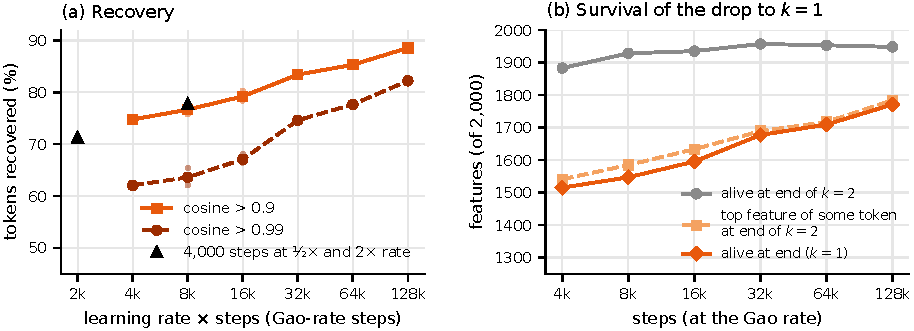
\includegraphics[width=\linewidth]{figures/topk_training.pdf}
\caption{TopK annealing on the 2k subset with more training. (a) Tokens recovered against learning rate times steps, in units of the Gao rate. Lines join runs at the Gao rate; small dots are single seeds where three were run. Triangles: 4,000 steps at half and twice the Gao rate. (b) Features alive at the end of the $k = 2$ stage, features that are some token's top feature at that point, and features alive at the end. The last two nearly coincide.}
\label{fig:topk-training}
\end{figure}

\subsection{The cost against ReLU}

TopK annealing works, but it is expensive. On the 2k subset, the best ReLU SAE recovered 98\% from about 8 million training examples (Section~\ref{sec:relu}). The best TopK run recovered 89\% from about 66 million (Figure~\ref{fig:headline}). That is eight times the training for less recovery. At about 3 points per doubling, matching 98\% would take several more doublings.

\section{ReLU SAEs with an L1 penalty: recovery across a wide region}
\label{sec:relu}

\subsection{The embeddings minimise the L1 loss}
\label{sec:relu-target}

We now turn from TopK to the other common architecture: a ReLU encoder with an L1 penalty. Here sparsity is not imposed by a hard limit on the number of active features. Instead, the penalty makes every active feature costly, and each token may use as many features as it likes. We first show that the embeddings are still the natural target, and then ask when training finds them.

With $\lambda > 0$, no dictionary reaches zero loss, because every active feature costs a penalty. The embeddings are still the natural target. The reason is a lower bound on the loss of each token.

\begin{proposition}\label{prop:l1}
For any unit-length dictionary and any non-negative code, the loss of a token $x$ with $\norm{x} > \lambda/2$ is at least $\lambda\norm{x} - \lambda^2/4$. A single feature along $x$, with coefficient $\norm{x} - \lambda/2$, reaches this bound.
\end{proposition}

The proof is short. By the triangle inequality, the penalty $\lambda\sum_j f_j$ is at least $\lambda\norm{\hat{x}}$. Among all reconstructions of a given length, the closest to $x$ points along $x$. Minimising over the length gives the bound. Appendix~\ref{app:l1} gives the argument step by step. The condition $\norm{x} > \lambda/2$ ensures that the optimal coefficient is positive. It is easily met here: the smallest GPT-2 embedding norm is 2.45, while $\lambda/2$ is at most 0.5 in our runs.

The optimal coefficient is $\norm{x} - \lambda/2$, not $\norm{x}$: the L1 penalty shrinks every coefficient by $\lambda/2$. This is the familiar shrinkage of the lasso \cite{tibshirani1996lasso}, which Gao et al.~\cite{gao2024scaling} also discuss for ReLU SAEs. Our full-scale run (Section~\ref{sec:fullscale}) shows exactly this: each token's coefficient ended at its norm minus 0.15, which is $\lambda/2$ for $\lambda = 0.3$.

With $m = V$, every token can have its own feature along it. Every token then sits at its lower bound at once, so the normalised embeddings minimise the total loss.

\subsection{One-hot codes are reachable for every GPT-2 token}
\label{sec:hull}

The argument assumes that the encoder can output this code exactly. Each token's own feature must be active, and every other feature must be zero on it. Whether this is possible is a geometric question about the embedding table. A ReLU encoder can do this for a token exactly when the token's embedding is a vertex of the convex hull of the table: a point that is not a weighted average of the other embeddings (Appendix~\ref{app:hull}). Every GPT-2 embedding is such a vertex. For 99.7\% of tokens the token's own direction already separates it from all the others, and a linear programme confirms the rest. So the minimiser is reachable in principle.

How widely a token is separated also predicts whether training finds it. We measure the \emph{own-direction margin}: how far the token's projection onto its own direction exceeds the largest projection of any other token, as a fraction of its norm. Figure~\ref{fig:margin} plots recovery in the full-scale ReLU run against this margin. Tokens with a margin above 0.3 are recovered almost without exception. Tokens with a small margin are recovered less often. So the unrecovered tokens are those which the ReLU encoder needed to isolate through a narrow gap, which training did not find.

\begin{figure}[t]
\centering
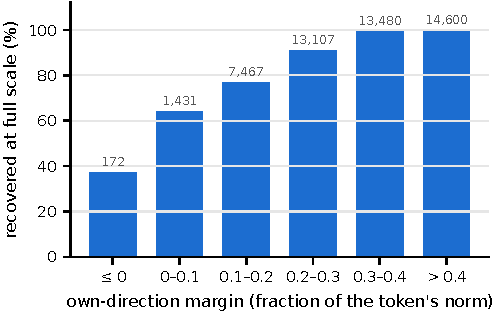
\includegraphics[width=0.58\linewidth]{figures/margin.pdf}
\caption{Recovery in the full-scale ReLU run ($\lambda = 0.3$, 93\% recovered overall) against each token's own-direction margin. The numbers above the bars are the number of tokens in each bin.}
\label{fig:margin}
\end{figure}

\subsection{Three regimes, and codes that end near one-hot}
\label{sec:regimes}

We mapped recovery on the 2k subset over the penalty $\lambda$ from 0.03 to 1, the learning rate from a quarter of the Gao rate to four times it, and the batch size from 256 to 4,096. Every run had the same 8 million training examples. Figure~\ref{fig:relu-grid} shows the results. There are three regimes.
\begin{itemize}[leftmargin=*]
\item \textbf{Undertrained: dense codes.} With a small $\lambda$, a low learning rate or too few steps, every feature stays alive, but tokens still use many features each. These runs are on the way to recovery and get there with more steps. This is a slow success, not a true failure.
\item \textbf{Successful.} Across $\lambda$ from 0.03 to 0.5, at learning rates up to the Gao rate, enough training recovers over 80\% of tokens. The best runs recovered 98\% ($\lambda = 0.03$), 95\% ($\lambda = 0.1$) and 88\% ($\lambda = 0.3$).
\item \textbf{Over-pressured: dead features.} A large $\lambda$ or a high learning rate kills features early, before they find a token (Figure~\ref{fig:relu-grid}c). At four times the Gao rate with $\lambda = 1$, only 3 to 7 features survive. These deaths happen early in training, and more training does not undo them. Recovery is then capped by the number of features alive.
\end{itemize}

\begin{figure}[t]
\centering
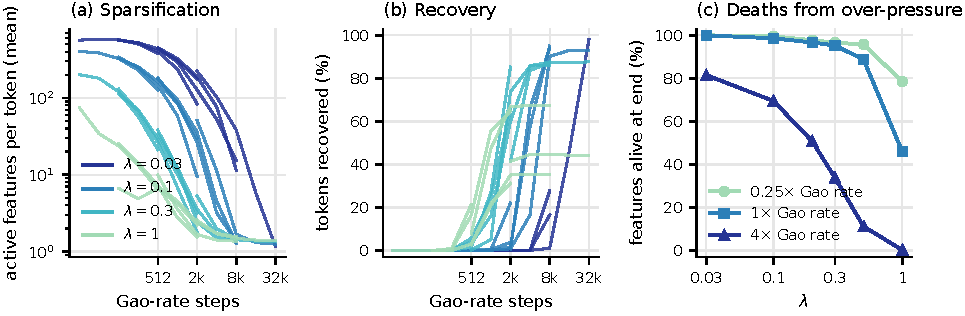
\includegraphics[width=\linewidth]{figures/relu_grid.pdf}
\caption{ReLU SAEs on the 2k subset. (a, b) Each line is one run at a quarter of the Gao rate or at the Gao rate, at batch size 256, 1,024 or 4,096. The horizontal axis is learning rate times steps, in units of the Gao rate. Runs with the same $\lambda$ follow similar curves whatever their batch size and learning rate. (c) Features alive at the end, averaged over the three batch sizes.}
\label{fig:relu-grid}
\end{figure}

Progress in the successful region depends on learning rate times steps, not on the batch size (Figure~\ref{fig:relu-grid}a, b). Runs with the same product reach similar sparsity, whatever their batch size. A plausible reason is that Adam moves each weight by about the learning rate per step. A larger batch gives a cleaner gradient, but no faster progress. Gao et al.~\cite{gao2024scaling} similarly find the batch size unimportant once the other settings are right.

Sparsification is gradual. Codes go from hundreds of active features per token to about one, one token at a time, while few features die. This is the contrast with TopK, where every token loses features at once at each drop. At full scale, codes went from about 25,000 active features per token to 1.37, while only about 400 of the 50,257 features died.

The codes end near one-hot, though not exactly (Figure~\ref{fig:codes}). Unlike TopK, a ReLU SAE lets each token use any number of features, so the number varies from token to token. In the best runs, 78\% to 90\% of tokens use a single feature, and a short tail uses more. The tokens that use two or more features are genuinely split between them. For these tokens, the second-largest coefficient is typically 34\% to 55\% of the largest, depending on the run, and it is below 10\% of the largest for at most 16\% of them. A feature with coefficient $f$ contributes roughly $(f/f_{\max})^2$ of a token's squared norm, so a typical second feature carries about 10\% to 30\% of it. This is why ignoring features with very small coefficients changes this picture little. With a cutoff at 10\% of the token's largest coefficient, the share of tokens on one feature moves by at most 2 points (Appendix~\ref{app:cutoff}).

\begin{figure}[t]
\centering
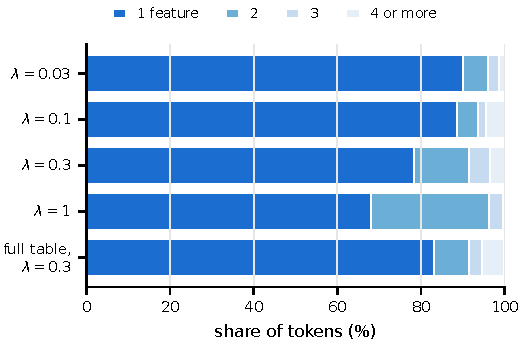
\includegraphics[width=0.6\linewidth]{figures/codes.pdf}
\caption{Active features per token at the end of the best ReLU run for each $\lambda$ on the 2k subset, and of the full-scale run. A feature is active if its coefficient is positive.}
\label{fig:codes}
\end{figure}

\subsection{The penalty must be weak, but not infinitely weak}
\label{sec:weak}

A smaller $\lambda$ recovers more, because it kills fewer features on the way to one-hot codes (Figure~\ref{fig:lambda}a). But a smaller $\lambda$ also sparsifies more slowly. Figure~\ref{fig:lambda}b measures the training needed until codes reach two active features per token on average. It grows roughly as $\lambda^{-0.9}$ between $\lambda = 0.03$ and 0.3: about 26,000 Gao-rate steps at $\lambda = 0.03$, against 2,000 to 4,000 at $\lambda = 0.3$. This is the ReLU form of the trade-off of Section~\ref{sec:tradeoff}.

So does $\lambda = 0$ do best of all? It recovers nothing (Figure~\ref{fig:nopenalty}a, b). With no penalty, every exact reconstruction has zero loss, so the bound of Proposition~\ref{prop:l1} no longer singles out the embeddings. The run reconstructs as well as the best penalised run, but with dense codes of about 670 features per token. For most of training it reconstructs better, since it pays nothing for using many features (Figure~\ref{fig:nopenalty}c). Its decoder rows stay close to random: the median cosine between a token and its nearest decoder row rises only from 0.12 to 0.16.

\begin{figure}[t]
\centering
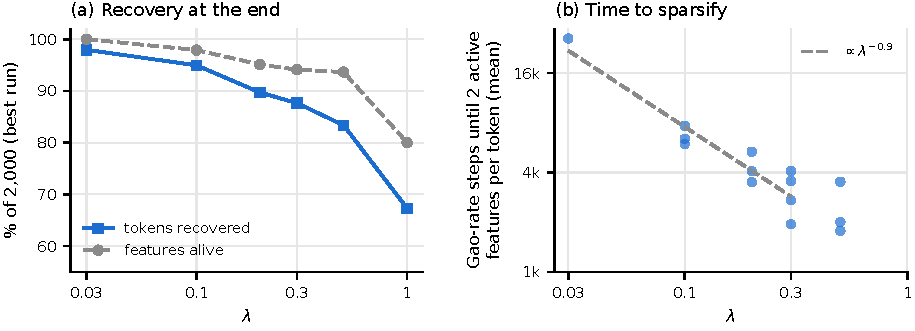
\includegraphics[width=\linewidth]{figures/lambda.pdf}
\caption{The strength of the penalty, on the 2k subset. (a) Tokens recovered and features alive at the end of the best run for each $\lambda$ in the grid (Table~\ref{tab:relu-grid}). (b) Training needed until codes reach two active features per token on average, for every run without heavy deaths. The dashed line is a fit for $\lambda \le 0.3$.}
\label{fig:lambda}
\end{figure}

\begin{figure}[t]
\centering
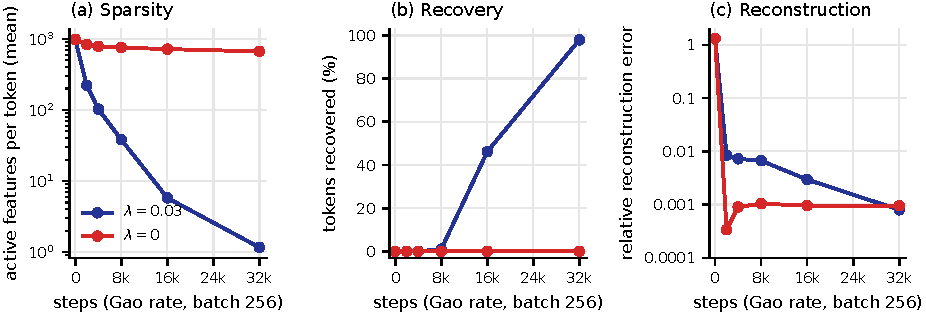
\includegraphics[width=\linewidth]{figures/no_penalty.pdf}
\caption{The same run on the 2k subset with $\lambda = 0.03$ and with no penalty (batch size 256, the Gao rate). The first point of each curve is the shared initialisation. (c) Squared reconstruction error relative to the squared norm of the tokens, without the penalty term. Without a penalty, the error falls by a factor of several thousand within 2,000 steps and then levels off at about 0.001. This floor is set by the constant learning rate: Adam's steps keep a size of about the learning rate, so the weights jitter around the minimum instead of settling on it.}
\label{fig:nopenalty}
\end{figure}

The picture is that the penalty must be weak, but not infinitely weak, and the training budget sets how weak. For any $\lambda > 0$, however small, the embeddings remain the minimiser of the loss. What shrinks as $\lambda$ falls is the force that pushes each code towards a single feature, so the time to sparsify grows. Only at $\lambda = 0$ itself does the minimiser disappear. The two sides of the trade-off are:
\begin{itemize}[leftmargin=*]
\item \textbf{Too strong:} features die before they find a token. On the 2k subset at the Gao rate, this sets in above about $\lambda = 0.5$.
\item \textbf{Too weak:} codes do not become sparse within the training available.
\end{itemize}
The best $\lambda$ is therefore roughly the smallest one that still finishes sparsifying in the time available. With unlimited training, a smaller $\lambda$ would keep doing better, right up to the discontinuity at zero.

\section{With training scaled to the vocabulary, recovery does not depend on its size}
\label{sec:sizes}

The results so far come mostly from the 2k subset. Do they carry over to larger vocabularies, and how must the settings change? We trained both architectures on the 5,000, 10,000 and 20,000 most frequent tokens, always with $m = V$. We ask two questions. First, how must the training budget grow with $V$ for recovery to stay the same? Second, do the best settings change with $V$: the penalty $\lambda$ for ReLU, and the starting $k_0$ for TopK?

\subsection{Measuring training across sizes}

To compare vocabularies of different sizes, we need a fair notion of ``the same amount of training''. A larger vocabulary has more tokens to learn and more features to train, so the same number of steps would not be a fair comparison.

Our rule is to scale the number of steps in proportion to $V$, at a fixed batch size. For example, a run of 4,000 steps on 2,000 tokens becomes a run of 40,000 steps on 20,000 tokens. Two measures of training are then the same at every size. The first is the number of steps per token of vocabulary, $S/V$. The second is the number of epochs' worth, $SB/V$: each token is seen the same number of times on average. The learning rate still follows the Gao rate, so it falls with size as $1/\sqrt{m}$. Larger vocabularies therefore get more steps, each with a smaller learning rate.

The two measures agree whenever the batch size is fixed, as in all the runs of the next two subsections. They differ only for the full-scale runs, which used larger batches (Section~\ref{sec:fullscale}). There we compare ReLU runs by steps per token, because at a fixed size the batch size hardly matters for ReLU (Section~\ref{sec:regimes}). We compare TopK runs by epochs' worth. A TopK feature gets gradient only when it is selected for a token in the minibatch, so the training it receives grows with the number of times each token is seen.

Our measure differs from the one used by Gao et al.~\cite{gao2024scaling}. They find that the number of training tokens needed for the loss to converge grows as about $m^{0.6}$. We measure the recovery of a fixed table, which each run sees many times over, rather than convergence on a stream of new activations.


\subsection{ReLU: recovery as a function of \texorpdfstring{$\lambda$}{lambda} is the same at every size}

Figure~\ref{fig:relu-sizes} trains each $\lambda$ for the same number of steps per token at every size. The curves for different sizes lie close together. At the end, each $\lambda$ recovers within a few points of the same share at all four sizes: 84\% to 89\% at $\lambda = 0.3$ and 90\% to 93\% at $\lambda = 0.1$. $\lambda = 1$ fails at every size, because about half the features die early. A smaller $\lambda$ recovers more at every size, given its longer training, so the best $\lambda$ does not change either.

This means the cheap map of Section~\ref{sec:regimes}, computed on 2,000 tokens, predicts what happens at larger sizes. The cost of a given recovery grows only in proportion to $V$, through the number of steps.

\begin{figure}[t]
\centering
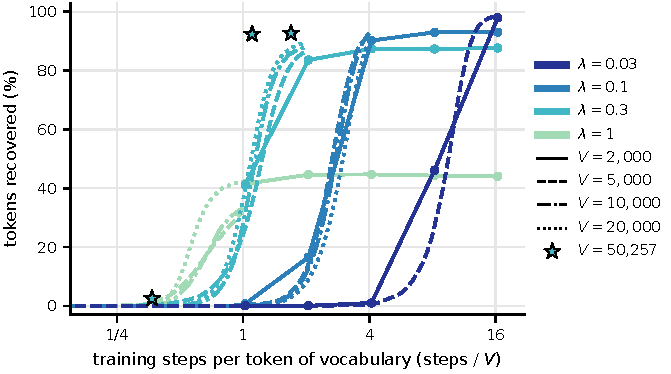
\includegraphics[width=0.85\linewidth]{figures/relu_sizes.pdf}
\caption{ReLU SAEs at four vocabulary sizes, at the Gao rate and batch size 256, against training steps divided by $V$. Colour gives $\lambda$ and line style gives the size. Each $\lambda$ runs for the same steps per token at every size; $\lambda = 0.03$ ran only at the two smallest sizes. Stars: the full-scale run at $\lambda = 0.3$ (batch size 1,024), measured three times during training.}
\label{fig:relu-sizes}
\end{figure}

\subsection{TopK: match the share alive at the start, and recovery is the same at every size}

For TopK, the starting $k_0$ must grow with the vocabulary. At the same $k$, fewer features are alive at initialisation in a larger vocabulary (Figure~\ref{fig:init}a). With 2,000 tokens, $k = 32$ leaves 93\% of features alive. With the full table, it leaves 77\%.

On the 2k subset, recovery levelled off once nearly every feature started alive. We therefore start each size at the $k_0$ that leaves 93\% of features alive at initialisation: 42, 55 and 71 at 5,000, 10,000 and 20,000 tokens. The schedule keeps the shape of Section~\ref{sec:anneal}, and the steps grow in proportion to $V$.

Recovery is then the same at every size (Figure~\ref{fig:topk-sizes}): 74\%, 75\% and 77\%, against 75\% on the 2k subset with the same training per token. The dynamics match too. Features die at the same drops and in the same proportions, and about 98\% of the survivors are recovered tokens.

The $k_0$ for 93\% alive follows a power law in $V$ (Figure~\ref{fig:init}b):
\begin{equation}
k_0 \approx 1.37\, V^{0.405} .
\end{equation}
This gives a recipe for carrying the schedule to any size. Start at the $k_0$ that leaves about 93\% of features alive, keep the shape of the schedule, and scale the steps in proportion to $V$.

\begin{figure}[t]
\centering
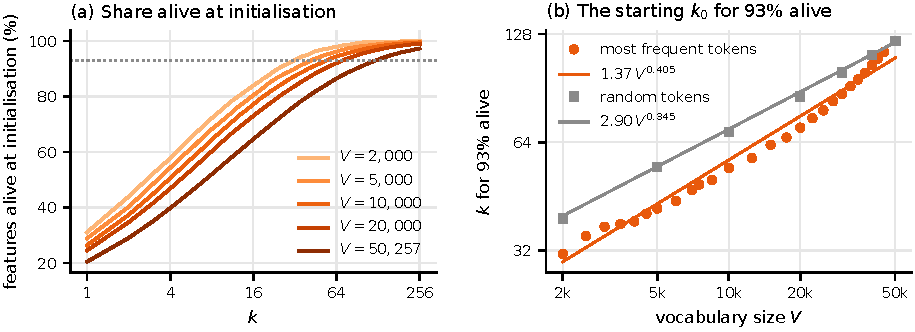
\includegraphics[width=\linewidth]{figures/init.pdf}
\caption{Features alive at initialisation, before any training. (a) Share of features that are among the top $k$ for some token, for subvocabularies of the most frequent tokens. The dotted line marks 93\%. (b) The $k$ that leaves 93\% alive, for subvocabularies of the most frequent tokens and of random tokens, with power-law fits. Means of two seeds.}
\label{fig:init}
\end{figure}

\begin{figure}[t]
\centering
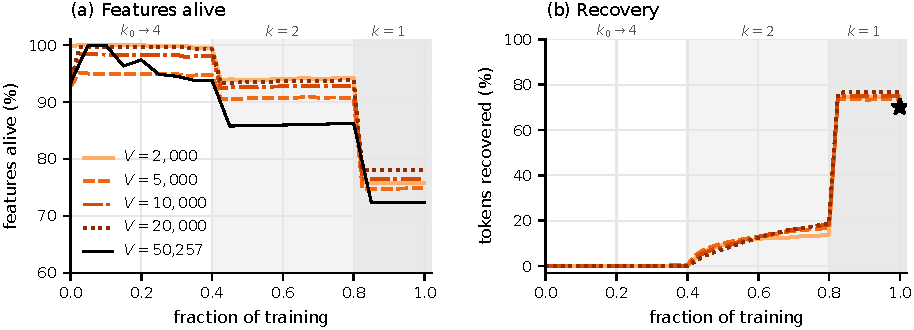
\includegraphics[width=\linewidth]{figures/topk_sizes.pdf}
\caption{TopK annealing at four vocabulary sizes with the same training per token (1,024 epochs' worth). Each size starts at the $k_0$ that leaves 93\% of features alive, except the 2k subset, which starts at 128 (99.8\% alive). Black: the full table, $k_0 = 128$ (93\% alive), about 1,300 epochs' worth. The star is its final recovery.}
\label{fig:topk-sizes}
\end{figure}

\subsection{The role of geometry}

Which tokens make up the vocabulary also matters. For random subsets of tokens, the $k$ for 93\% alive follows a cleaner power law with a smaller exponent, $2.90\,V^{0.345}$ (Figure~\ref{fig:init}b). The two curves meet at the full table.

The difference comes from the geometry of the embeddings. GPT-2's embeddings share a common direction, as is typical of language-model representations \cite{ethayarajh2019contextual}. Frequent tokens are spread more evenly around it than rare ones: the mean pairwise cosine is 0.24 for the 2,000 most frequent tokens, 0.27 for 2,000 random tokens and 0.34 for the 2,000 rarest. Evenly spread tokens are easier to cover, because different random features win different tokens. As a frequency subvocabulary grows, it adds rarer tokens that crowd closer together, so the $k_0$ it needs rises faster than size alone would make it.

This crowding does not make tokens harder to isolate, however. The own-direction margin of Section~\ref{sec:hull} barely changes with size. From 2,000 tokens to the full table, the median margin falls only from 0.36 to 0.32. So differences in recovery across sizes come from training, not from tokens becoming harder to separate.

\subsection{Full scale}
\label{sec:fullscale}

Both architectures were also trained once on the full table, before the size runs.

The annealed TopK SAE recovered 70\% after about 1,300 epochs' worth (Figure~\ref{fig:topk-sizes}). The smaller vocabularies recover 74\% to 77\% after 1,024 epochs' worth, and the full table loses features at the same drops (Figure~\ref{fig:topk-sizes}a). The full table started with 93\% of features alive at $k_0 = 128$, like the smaller sizes.

The ReLU SAE with $\lambda = 0.3$ recovered 93\% (Figure~\ref{fig:relu-sizes}, stars), against 84\% to 89\% for the smaller vocabularies at the end of their shorter runs. It got there in fewer steps per token than they did: it had 92\% after 1.1 steps per token, where the smaller vocabularies had about 35\% to 50\%. It used batch size 1,024 rather than 256, and larger vocabularies were already slightly ahead of smaller ones in Figure~\ref{fig:relu-sizes}. So steps in proportion to $V$ is a safe budget rather than an exact law: at full scale it overestimates the training needed.

\section{Discussion}
\label{sec:discussion}

We suggest possible explanations for our empirical findings.

\paragraph{Why is TopK so much slower?} A ReLU SAE sparsifies gradually. Each token sheds features at its own pace, and a feature that loses one token can keep or find others. A TopK schedule removes slots from every token at the same moment. At each drop, every feature that is not among the top $k$ for some token dies at once, and it has no way back. More training helps only by sorting features into their tokens before the drop. This may be why TopK keeps gaining from training long after ReLU has converged.

\paragraph{What might carry over to activations?} Real SAEs are trained on activations, with far more features than dimensions and no known target. Two of our lessons seem likely to carry over. First, dead features in TopK SAEs may come from competition for slots rather than from a lack of gradient, and auxiliary losses aimed at the gradient will then do little. Second, the training budget, not only the penalty, decides the best L1 coefficient. The scale independence of Section~\ref{sec:sizes} also suggests that cheap small-scale sweeps can be trusted, if training is scaled with the number of features.

\section{Limitations}
\label{sec:limitations}

\paragraph{One table, one model.} All results use the input embedding table of GPT-2 Small. The embeddings are a few tens of thousands of points in 768 dimensions, all of them hull vertices. Activations have more features than dimensions, and a different geometry.

\paragraph{Seeds.} Most runs use one seed. Repeated runs suggest a single run is good to about $\pm1$ percentage point on the 2k subset. We read no conclusion from differences of that size.

\paragraph{Training length.} We stopped the TopK runs at 128,000 steps, while recovery was still rising, so their limit is unknown. The ReLU runs at $\lambda = 0.1$ were also still rising at the end at every size, so their numbers are lower bounds.

\paragraph{Settings.} The learning rate follows a scaling derived for TopK SAEs on activations, which we also use for ReLU SAEs. We did not tune it per architecture beyond the grid of Section~\ref{sec:regimes}. The subvocabularies are chosen by frequency, which changes their geometry as they grow. The recovery thresholds of 0.9 and 0.99 are our choice.

\section{Related work}
\label{sec:related}

\paragraph{Sparse autoencoders.} Sparse coding and dictionary learning have a long history \cite{olshausen1996emergence,aharon2006ksvd}. SAEs with an L1 penalty were applied to language-model activations by Cunningham et al.~\cite{cunningham2023sparse} and Bricken et al.~\cite{bricken2023monosemanticity}, and scaled up by Templeton et al.~\cite{templeton2024scaling}. Gao et al.~\cite{gao2024scaling} replaced the L1 penalty by a TopK activation, following the $k$-sparse autoencoders of Makhzani and Frey~\cite{makhzani2013ksparse}. They also gave scaling laws, the AuxK loss and the learning-rate scaling we use. Other variants include gated \cite{rajamanoharan2024gated}, JumpReLU \cite{rajamanoharan2024jumprelu} and BatchTopK SAEs \cite{bussmann2024batchtopk}. BatchTopK fixes the number of active features per batch rather than per input, which allows codes of variable length like those of our ReLU SAEs. Nelson et al.~\cite{nelson2026identifiable} show that TopK SAEs trained from different seeds learn different dictionaries and codes. They connect SAEs to classical dictionary learning and propose variants whose codes are identifiable.

\paragraph{Dead features and shrinkage.} Dead features have been addressed by resampling \cite{bricken2023monosemanticity}, ghost gradients \cite{jermyn2024ghost} and AuxK \cite{gao2024scaling}. The shrinkage caused by an L1 penalty is studied by Wright and Sharkey~\cite{wright2024suppression}. Our setting isolates both effects against a known target.

\paragraph{Sparse codes for static word embeddings.} Sparse autoencoders have been applied to static word embeddings before. SPINE \cite{subramanian2018spine} trains a sparse autoencoder on GloVe and word2vec vectors, with 1,000 hidden dimensions for 15,000 words, to obtain more interpretable coordinates. Its aim is interpretable shared dimensions, not reproducing each input vector. Templeton~\cite{templeton2020word} codes word embeddings sparsely in a dictionary built from word-embedding directions. There the dictionary is fixed in advance rather than learned, so the question of whether training finds it does not arise.

\paragraph{SAEs and the vocabulary.} The closest work is VASAE \cite{zhang2026vasae}. It trains TopK SAEs ($k = 32$) with exactly vocabulary-sized dictionaries on the contextual residual stream of GPT-2 Small and Llama 3.1 8B. The decoder rows of an ordinary SAE stay far from the token embeddings, with nearest-token cosines of about 0.1 to 0.2. A soft penalty that pulls them towards the embeddings aligns most of them, though not one-to-one. A decoder fixed to the embeddings reconstructs the residual stream poorly. So having $m = V$ does not by itself make an SAE on contextual activations find the embeddings. Our setting asks the same question when the training data are the raw embeddings themselves. Other work studies SAE features tied to single tokens in contextual activations, and finds that their causal role depends on how the SAE was trained \cite{cho2026singletoken}. Even the earliest residual stream differs from the raw embedding table, because it adds position embeddings \cite{chughtai2024positional}. SAEs on the token representations of a clinical language model find features shared by related tokens rather than one feature per token \cite{wu2024beyond}.

\paragraph{One-sparse dictionary learning and clustering.} With one non-zero coefficient per input and unit-length dictionary elements, dictionary learning becomes gain-shape vector quantisation, closely related to spherical $k$-means \cite{coates2012kmeans}. There the codes are optimised directly for each input, whereas a Top1 SAE must output them from a learned encoder. Heimersheim and Engels~\cite{heimersheim2024shortform} discuss informally whether a well-trained Top1 SAE should match a clustering of its inputs, with experiments on contextual activations.

\paragraph{Known ground truth.} Sharkey et al.~\cite{sharkey2022taking} tested SAEs on synthetic data with known features, and Elhage et al.~\cite{elhage2022toy} study toy models of superposition. Theoretical work gives conditions under which dictionary learning recovers a true dictionary \cite{spielman2012exact,arora2014new}. Closer to SAEs, Rangamani et al.~\cite{rangamani2017sparse} study when a shallow ReLU autoencoder recovers the dictionary of a sparse-coding model, and Nguyen et al.~\cite{nguyen2019dynamics} prove that gradient descent recovers the parameters of weight-sharing autoencoders under sparse generative models. Our setting uses real data with a known answer, and asks whether standard SAE training finds it from random initialisation. Chanin et al.~\cite{chanin2024absorption} measure how SAE features on activations depart from known features, such as the first letter of a token.

\section{Conclusion}

With one feature per token and no bottleneck, an SAE trained on GPT-2's embedding table has a known target: the embeddings themselves. Training can find it with either architecture, but the architecture decides which regimes work and how much training they cost. A ReLU SAE with an L1 penalty recovers 93\% to 98\% of tokens across a wide region of settings, provided the penalty is weak but not zero and training is long enough. A TopK SAE fails with any fixed $k$. Annealing $k$ to 1 succeeds, at a cost far above ReLU's, because every drop in $k$ is a contest that some features lose for good. For both architectures, recovery depends on the training per token and not on the vocabulary size. So small, cheap experiments predict the full-scale behaviour.

Natural next steps are longer TopK runs to find where annealing levels off, and the same test on synthetic data with a planted dictionary. Such data would be built from a chosen set of feature directions, more of them than dimensions as in superposition, with each vector a sparse non-negative combination of them \cite{sharkey2022taking}. This keeps a known answer, as here, while adding the bottleneck that our setting deliberately leaves out.

\section*{Acknowledgements}

Beyond the initial project design, this project's code, analysis and this write-up were developed in collaboration with Claude (Anthropic).

\bibliographystyle{alpha}
\bibliography{refs}

\clearpage
\appendix

\section{Why the embeddings minimise the L1 loss}
\label{app:l1}

This appendix proves Proposition~\ref{prop:l1}.

\paragraph{Setup.} Take one token $x$. The SAE reconstructs it as $\hat{x} = \sum_j f_j d_j$, with coefficients $f_j \ge 0$ and unit-length decoder rows, $\norm{d_j} = 1$. Its loss is
\begin{equation}
L = \norm{x - \hat{x}}^2 + \lambda \sum_j f_j .
\end{equation}

\paragraph{Step 1: the penalty is at least the length of the reconstruction.} By the triangle inequality,
\begin{equation}
\norm{\hat{x}} = \Big\lvert \sum_j f_j d_j \Big\rvert \le \sum_j f_j \norm{d_j} = \sum_j f_j .
\end{equation}
So $L \ge \norm{x - \hat{x}}^2 + \lambda\norm{\hat{x}}$. This bound depends only on the vector $\hat{x}$, not on how it was built.

\paragraph{Step 2: the best possible reconstruction.} Say $\hat{x}$ has length $t$. Among all vectors of length $t$, the one closest to $x$ points along $x$, so the error is at least $(\norm{x} - t)^2$. Therefore
\begin{equation}
L \ge h(t) = (\norm{x} - t)^2 + \lambda t .
\end{equation}
The derivative is $h'(t) = -2(\norm{x} - t) + \lambda$, which is zero at $t = \norm{x} - \lambda/2$. There,
\begin{equation}
h = \left(\frac{\lambda}{2}\right)^2 + \lambda\left(\norm{x} - \frac{\lambda}{2}\right) = \lambda\norm{x} - \frac{\lambda^2}{4} .
\end{equation}
This is a lower bound on the token's loss, whatever the dictionary and whatever the code. It assumes $\norm{x} > \lambda/2$, which holds here: the smallest GPT-2 embedding norm is 2.45.

The minimum is not at full length. At $t = \norm{x}$ the loss is $\lambda\norm{x}$, but $h'(\norm{x}) = \lambda > 0$, so shrinking the reconstruction slightly lowers it. Shortening saves penalty at rate $\lambda$, while the squared error grows from zero only quadratically. For example, with $\norm{x} = 4$ and $\lambda = 0.3$, the full-length reconstruction has loss $0 + 1.2 = 1.2$. The reconstruction shortened by $\lambda/2$ has loss $0.0225 + 1.155 = 1.1775$.

\paragraph{Step 3: one feature pointing at the token reaches the bound.} Use the single feature $d = x/\norm{x}$ with coefficient $f = \norm{x} - \lambda/2$. The reconstruction is $x$ shortened by $\lambda/2$, so the error is $(\lambda/2)^2$. The penalty is $\lambda(\norm{x} - \lambda/2)$. They add to $\lambda\norm{x} - \lambda^2/4$, which is exactly the bound.

\paragraph{Conclusion.} No code can do better for a token than a single feature pointing along it, with coefficient $\norm{x} - \lambda/2$. With $m = V$, every token can have its own such feature. Every token then sits at its lower bound at once, and the normalised embeddings minimise the total loss. The only assumption is that the ReLU encoder can output this code exactly: the token's own feature active, and every other feature at zero. Appendix~\ref{app:hull} turns this assumption into a geometric condition.

\paragraph{No penalty.} At $\lambda = 0$ the bound is zero. Every dictionary that spans the embeddings, with any code that reconstructs them exactly, reaches it. So the loss no longer prefers the embeddings, and nothing in training pulls the features towards them.

\section{When can a ReLU encoder output one-hot codes?}
\label{app:hull}

\paragraph{What is needed.} The encoder computes $f_j = \mathrm{ReLU}(w_j \cdot x + b_j)$, with an encoder row $w_j$ and a bias $b_j$ for each feature. Assign feature $j$ to token $j$. The code of Appendix~\ref{app:l1} requires two things of feature $j$:
\begin{itemize}[leftmargin=*]
\item On its own token, $w_j \cdot x_j + b_j = \norm{x_j} - \lambda/2$, which is positive.
\item On every other token, $w_j \cdot x_i + b_j \le 0$ for all $i \ne j$, so that the ReLU outputs zero.
\end{itemize}

\paragraph{Step 1: the condition splits into one question per token.} The encoder is not tied to the decoder, so each pair $(w_j, b_j)$ can be chosen on its own. The two requirements on feature $j$ say that the hyperplane $w_j \cdot x + b_j = 0$ has $x_j$ strictly on its positive side and every other token on or behind it.

\paragraph{Step 2: the scale is free.} Suppose some pair $(w, b)$ separates $x_j$ in this way, with $w \cdot x_j + b = s > 0$. Multiply both $w$ and $b$ by $(\norm{x_j} - \lambda/2)/s$. Every other token stays on or behind the hyperplane, and the coefficient on $x_j$ becomes exactly $\norm{x_j} - \lambda/2$. So feature $j$ can produce the required code exactly when some hyperplane separates $x_j$ from the other tokens. The value of $\lambda$ plays no part.

\paragraph{Step 3: separable means a vertex of the convex hull.} A point can be separated from a finite set of points exactly when it is not a weighted average, or convex combination, of them (Figure~\ref{fig:hull}). One direction is short. Suppose $x_j = \sum_{i \ne j} c_i x_i$ with $c_i \ge 0$ and $\sum_i c_i = 1$. Then for any $w$ and $b$,
\begin{equation}
w \cdot x_j + b = \sum_{i \ne j} c_i\,(w \cdot x_i + b) \le 0 ,
\end{equation}
since every term in the sum is at most zero. So the coefficient on $x_j$ cannot be positive. The other direction is the separating hyperplane theorem. A token that is not a weighted average of the others is a vertex of the convex hull of the table.

\begin{figure}[h]
\centering
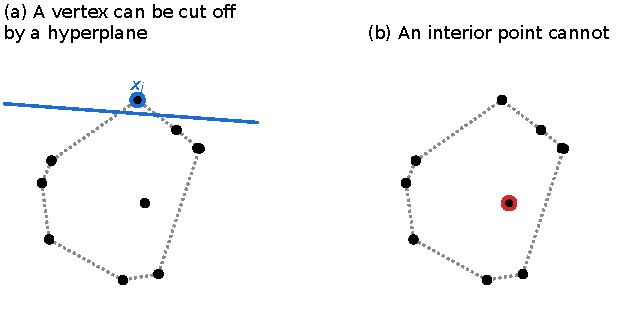
\includegraphics[width=0.6\linewidth]{figures/hull.pdf}
\caption{A two-dimensional illustration. (a) A point on the corner of the hull can be cut off from the others by a line, so a ReLU feature can fire on it alone. (b) A point inside the hull cannot: any line with it on the positive side also has some other point there.}
\label{fig:hull}
\end{figure}

\paragraph{Conclusion.} One-hot codes are possible for exactly the tokens whose embeddings are vertices of the convex hull of the table. If every embedding is a vertex, the minimiser of Appendix~\ref{app:l1} is reachable. A token that is not a vertex can never have a feature of its own. It must be coded as a mixture of features, at a loss above its bound.

\paragraph{How to check it.} We use two tests, from cheap to exact.
\begin{enumerate}[leftmargin=*]
\item \textbf{The own-direction test} is sufficient. Take $w_j = x_j/\norm{x_j}$. This separates $x_j$ if no other token projects further along $x_j$'s direction than $x_j$ itself: $\max_{i \ne j} w_j \cdot x_i < \norm{x_j}$. The bias then sits between the two values. The \emph{own-direction margin} is $(\norm{x_j} - \max_{i \ne j} w_j\cdot x_i)/\norm{x_j}$.
\item \textbf{The linear-programme test} is exact. For a token that fails the first test, a different direction may still separate it. A linear programme decides whether any separating hyperplane exists. It has 769 unknowns, $w_j$ and $b_j$, and one constraint per other token. We bound each coordinate of $w$ by 1 and maximise $w \cdot x_j + b$. Constraints are added in rounds: the 2,000 tokens that project furthest along $x_j$'s direction come first, then any violated constraints, until none remain. We solve it with HiGHS \cite{huangfu2018highs} in SciPy \cite{virtanen2020scipy}.
\end{enumerate}

The first test differs from a tied encoder. With $w_j$ tied to the decoder row $x_j/\norm{x_j}$, the coefficient on $x_j$ forces $b_j = -\lambda/2$. Every other token then needs $w_j \cdot x_i \le \lambda/2$, which is far stricter and depends on $\lambda$. Our SAEs have untied encoders, so only the hull condition matters.

\paragraph{Results for GPT-2.} Table~\ref{tab:hull} gives the results. Every embedding is a vertex of the hull. The 172 tokens of the full table that fail the own-direction test fall into two groups. 115 of them have a linear-programme margin of 0.32 to 0.40: they are well separated, just not along their own direction. The full-scale ReLU run recovered 63 of them. The other 57 have a margin of about 0.04, and 56 of them never occur in our Wikipedia count, so they are probably unused tokens. The full-scale run recovered one of them. Table~\ref{tab:margin} gives the recovery by margin plotted in Figure~\ref{fig:margin}.

\begin{table}[h]
\centering
\begin{tabular}{lrr}
\toprule
Test & Full table & 2k subset \\
\midrule
Pass the own-direction test & 50,085 & 1,999 \\
Fail it, but separable by the linear programme & 172 & 1 \\
Not separable & 0 & 0 \\
\bottomrule
\end{tabular}
\caption{The convex-hull check for GPT-2.}
\label{tab:hull}
\end{table}

\begin{table}[h]
\centering
\begin{tabular}{lrr}
\toprule
Own-direction margin & Tokens & Recovered at full scale \\
\midrule
0 or below (test fails) & 172 & 37\% \\
0 to 0.1 & 1,431 & 64\% \\
0.1 to 0.2 & 7,467 & 77\% \\
0.2 to 0.3 & 13,107 & 91\% \\
0.3 to 0.4 & 13,480 & 99.3\% \\
Above 0.4 & 14,600 & 100\% \\
\bottomrule
\end{tabular}
\caption{Recovery in the full-scale ReLU run ($\lambda = 0.3$) by own-direction margin.}
\label{tab:margin}
\end{table}

\section{Training setup}
\label{app:setup}

\paragraph{Common to every run.}
\begin{itemize}[leftmargin=*]
\item \textbf{Data.} The rows of the GPT-2 Small input embedding table, or of a subvocabulary of its $V$ most frequent tokens. Frequency is counted on about 200 million tokens of English Wikipedia (snapshot \texttt{20231101.en}) and only decides which tokens make up a subvocabulary.
\item \textbf{Sampling.} Each minibatch is drawn uniformly at random from the vocabulary, with replacement. There is no frequency weighting.
\item \textbf{Steps and epochs.} A step is one optimiser update on one minibatch. With $V$ tokens and batch size $B$, one epoch's worth of examples goes by every $V/B$ steps. Sampling is with replacement, so these are not exact passes through the vocabulary.
\item \textbf{Model.} $m = V$ features. Decoder rows have unit norm. They are kept so by removing the gradient component along each row before the update and renormalising after it. No decoder bias. Random Gaussian decoder rows, the encoder initialised as the transpose of the decoder, and zero encoder bias.
\item \textbf{Optimiser.} Adam with default settings and a constant learning rate. The Gao rate is $2\times10^{-4}/\sqrt{m/2^{14}}$ (Table~\ref{tab:gao}). The $1/\sqrt{m}$ scaling follows Gao et al.~\cite{gao2024scaling}. The constant is our own normalisation.
\item \textbf{Evaluation.} Over every token of the vocabulary, weighted equally. A token is recovered if some decoder row is its mutual nearest neighbour at a cosine above 0.9 (or 0.99). A feature is alive if it is active on at least one token, and active on a token if its coefficient is positive.
\item \textbf{Seeds and hardware.} One seed per run, except two lengths of TopK annealing with three seeds (Table~\ref{tab:topk}). Runs used PyTorch \cite{paszke2019pytorch} on CPUs: the full-scale and size runs on a laptop, and most 2k-subset pilots in a cloud sandbox.
\end{itemize}

\begin{table}[h]
\centering
\begin{tabular}{lccccc}
\toprule
$m = V$ & 2,000 & 5,000 & 10,000 & 20,000 & 50,257 \\
\midrule
Gao rate & $5.7\times10^{-4}$ & $3.6\times10^{-4}$ & $2.6\times10^{-4}$ & $1.8\times10^{-4}$ & $1.1\times10^{-4}$ \\
\bottomrule
\end{tabular}
\caption{The Gao rate at each vocabulary size.}
\label{tab:gao}
\end{table}

\begin{table}[h]
\centering
\small
\begin{tabular}{@{}L{2.7cm}L{2.9cm}L{1.6cm}L{2.9cm}cL{1.9cm}@{}}
\toprule
Runs & Model & $V$ & Steps (batch) & LR & Epochs' worth \\
\midrule
Fixed $k$ & TopK & 2,000 & 3,000 (512) & 1 & 768 \\
Annealing pilots, AuxK & TopK & 2,000 & 4,000 (512) & 1 & 1,024 \\
Top1, full table & TopK, $k = 1$ & 50,257 & 16,820 (4,096) & 1 & 1,371 \\
Annealing, full table & TopK, $k_0 = 128$ & 50,257 & 15,980 (4,096) & 1 & 1,302 \\
More training & TopK, $k_0 = 128$ & 2,000 & 4,000 to 128,000 (512) & $\tfrac12$, 1, 2 & 1,024 to 32,768 \\
Sizes & TopK, $k_0$ = 42, 55, 71 & 5k, 10k, 20k & $2V$ (512) & 1 & 1,024 \\
ReLU grid & ReLU, $\lambda$ = 0.03 to 1 & 2,000 & 32,768; 8,192; 2,048 (256; 1,024; 4,096) & $\tfrac14$, 1, 4 & 4,194 \\
No penalty & ReLU, $\lambda = 0$ & 2,000 & 32,768 (256) & 1 & 4,194 \\
ReLU, full table & ReLU, $\lambda = 0.3$ & 50,257 & 85,100 (1,024) & 1 & 1,734 \\
Sizes & ReLU, $\lambda$ = 1, 0.3, 0.1 (0.03) & 5k, 10k, 20k & $V$, $2V$, $4V$ ($16V$) (256) & 1 & 256, 512, 1,024 (4,096) \\
\bottomrule
\end{tabular}
\caption{The training runs. LR is the learning rate as a multiple of the Gao rate. The annealed TopK runs use the schedule with a long $k = 2$ stage unless stated otherwise in Table~\ref{tab:topk}. At the sizes, $\lambda = 0.03$ ran only at 5,000 tokens.}
\label{tab:runs}
\end{table}

\clearpage
\section{Full results}
\label{app:results}

\begin{table}[h]
\centering
\small
\begin{tabular}{@{}p{7.2cm}rrr@{}}
\toprule
Run & Alive & Rec.\ $>0.9$ & Rec.\ $>0.99$ \\
\midrule
\multicolumn{4}{l}{\emph{Fixed $k$}} \\
Top1, full table & 259 & 16 (0.03\%) & 6 \\
Top1 & 382 & 227 (11\%) & 113 \\
Fixed $k$ = 2, 4, 8, 16, 32 (3,000 steps) & 558--1,778 & 162, 73, 7, 0, 0 & 13, 0, 0, 0, 0 \\
\midrule
\multicolumn{4}{l}{\emph{Annealing (4,000 steps)}} \\
2 for 80\%, then 1 & 545 & 295 (15\%) & 136 \\
4 for 20\%, 2 for 60\%, then 1 & 750 & 506 (25\%) & 250 \\
Halving from $k_0$ = 8 & 1,025 & 851 (43\%) & 530 \\
Halving from $k_0$ = 16 & 1,265 & 1,171 (59\%) & 849 \\
Halving from $k_0$ = 32 & 1,414 & 1,362 (68\%) & 1,068 \\
Halving from $k_0$ = 64 & 1,482 & 1,454 (73\%) & 1,184 \\
Halving from $k_0$ = 128 & 1,474 & 1,438 (72\%) & 1,171 \\
Long $k = 2$ stage from $k_0$ = 32 & 1,441 & 1,402 (70\%) & 1,115 \\
Long $k = 2$ stage from $k_0$ = 64 & 1,532 & 1,501 (75\%) & 1,267 \\
Long $k = 2$ stage from $k_0$ = 128 & 1,523 & 1,499 (75\%) & 1,250 \\
Long $k = 2$ stage from $k_0$ = 128, full table & 36,354 & 35,261 (70\%) & 28,502 (57\%) \\
\midrule
\multicolumn{4}{l}{\emph{Annealing with AuxK (long $k = 2$ stage from 128, 4,000 steps)}} \\
Standard AuxK, weight 1/32, 1/8 & 1,507; 1,516 & 1,476; 1,478 & 1,229; 1,235 \\
Whole-token AuxK, weight 1/32, 1/8, 1/2 & 1,525--1,555 & 1,503; 1,542; 1,538 & 1,258--1,304 \\
\midrule
\multicolumn{4}{l}{\emph{More training (long $k = 2$ stage from 128)}} \\
4,000 steps at $\tfrac12\times$ Gao rate & 1,479 & 1,426 (71\%) & 1,187 \\
4,000 steps & 1,515 & 1,495 (75\%) & 1,241 \\
8,000 steps, mean of 3 seeds & 1,547 & 1,533 (77\%) & 1,272 \\
4,000 steps at $2\times$ Gao rate & 1,553 & 1,555 (78\%) & 1,300 \\
16,000 steps, mean of 3 seeds & 1,595 & 1,584 (79\%) & 1,341 \\
32,000 steps & 1,677 & 1,668 (83\%) & 1,492 \\
64,000 steps & 1,709 & 1,706 (85\%) & 1,553 \\
128,000 steps & 1,771 & 1,771 (89\%) & 1,644 \\
\midrule
\multicolumn{4}{l}{\emph{Sizes (1,024 epochs' worth)}} \\
$k_0 = 42$, 5,000 tokens & 3,741 & 3,678 (74\%) & 2,993 (60\%) \\
$k_0 = 55$, 10,000 tokens & 7,642 & 7,512 (75\%) & 6,158 (62\%) \\
$k_0 = 71$, 20,000 tokens & 15,604 & 15,370 (77\%) & 12,826 (64\%) \\
\bottomrule
\end{tabular}
\caption{All TopK runs, on the 2k subset unless stated otherwise. Every annealed run ends at $k = 1$, so every token uses exactly one feature at the end. The 8,000- and 16,000-step seeds range over 1,515 to 1,555 and 1,568 to 1,606 recovered tokens.}
\label{tab:topk}
\end{table}

\begin{table}[h]
\centering
\small
\begin{tabular}{lrrrrrrrrr}
\toprule
& \multicolumn{3}{c}{Batch 256} & \multicolumn{3}{c}{Batch 1,024} & \multicolumn{3}{c}{Batch 4,096} \\
\cmidrule(lr){2-4}\cmidrule(lr){5-7}\cmidrule(lr){8-10}
$\lambda$ & $\tfrac14$ & 1 & 4 & $\tfrac14$ & 1 & 4 & $\tfrac14$ & 1 & 4 \\
\midrule
0.03 & 330 & \textbf{1,959} & 1,372 & 1 & 555 & 1,065 & 0 & 1 & 321 \\
0.1 & 1,881 & 1,861 & 1,128 & 440 & \textbf{1,899} & 1,190 & 3 & 75 & 827 \\
0.2 & 1,793 & 1,794 & 760 & 1,632 & 1,788 & 762 & 17 & 945 & 748 \\
0.3 & 1,724 & \textbf{1,753} & 430 & 1,705 & 1,751 & 384 & 77 & 1,315 & 399 \\
0.5 & 1,667 & 1,640 & 51 & 1,631 & 1,612 & 27 & 302 & 1,438 & 35 \\
1 & \textbf{1,346} & 881 & 0 & 1,296 & 709 & 0 & 428 & 626 & 0 \\
\bottomrule
\end{tabular}
\caption{The ReLU grid on the 2k subset: tokens recovered (of 2,000) at a cosine above 0.9 after 8 million training examples, by $\lambda$, batch size and learning rate as a multiple of the Gao rate. Bold: the best cell for each $\lambda$ shown in Figure~\ref{fig:codes}.}
\label{tab:relu-grid}
\end{table}

\begin{table}[h]
\centering
\small
\begin{tabular}{lrrrrrrr}
\toprule
& & & \multicolumn{4}{c}{Share of tokens using} & \\
\cmidrule(lr){4-7}
Run & Recovered & Mean & 1 & 2 & 3 & 4+ & Max \\
\midrule
$\lambda = 0.03$, 2k subset & 1,959 (98\%) & 1.16 & 90.1\% & 5.9\% & 2.7\% & 1.4\% & 6 \\
$\lambda = 0.1$, 2k subset & 1,899 (95\%) & 1.27 & 88.5\% & 5.0\% & 2.1\% & 4.5\% & 10 \\
$\lambda = 0.3$, 2k subset & 1,753 (88\%) & 1.35 & 78.4\% & 13.1\% & 5.0\% & 3.6\% & 6 \\
$\lambda = 1$, 2k subset & 1,346 (67\%) & 1.36 & 68.1\% & 28.2\% & 3.3\% & 0.5\% & 5 \\
$\lambda = 0.3$, full table & 46,590 (93\%) & 1.37 & 83.2\% & 8.3\% & 3.0\% & 5.4\% & 11 \\
$\lambda = 0$, 2k subset & 0 (0\%) & 668 & & & & & \\
\bottomrule
\end{tabular}
\caption{Active features per token at the end of the best ReLU run for each $\lambda$, and of the full-scale and no-penalty runs. The full-scale run recovered 44,337 tokens (88\%) at a cosine above 0.99, with 49,869 features alive, after 85,100 steps.}
\label{tab:relu-best}
\end{table}

\begin{table}[h]
\centering
\small
\begin{tabular}{lrrrrr}
\toprule
$\lambda$ & Epochs' worth & 2,000 & 5,000 & 10,000 & 20,000 \\
\midrule
1 & 256 & 830 (42\%) & 1,587 (32\%) & 3,291 (33\%) & 8,442 (42\%) \\
0.3 & 512 & 1,672 (84\%) & 4,333 (87\%) & 8,799 (88\%) & 17,867 (89\%) \\
0.1 & 1,024 & 1,804 (90\%) & 4,604 (92\%) & 9,262 (93\%) & 18,033 (90\%) \\
0.03 & 4,096 & 1,959 (98\%) & 4,925 (98.5\%) & & \\
\bottomrule
\end{tabular}
\caption{ReLU SAEs at four vocabulary sizes, at the Gao rate and batch size 256: tokens recovered at a cosine above 0.9. The 2,000-token column is read from the ReLU grid at the nearest epochs' worth (262, 524, 1,049 and 4,194).}
\label{tab:relu-sizes}
\end{table}

\begin{table}[h]
\centering
\small
\begin{tabular}{lrrrrrr}
\toprule
$V$ & $k = 1$ & 8 & 32 & 64 & 128 & 256 \\
\midrule
2,000 & 31\% & 72\% & 93\% & 98\% & 99.8\% & 100\% \\
5,000 & 29\% & 68\% & 90\% & 96\% & 98.9\% & 99.8\% \\
10,000 & 26\% & 65\% & 88\% & 95\% & 98.1\% & 99.6\% \\
20,000 & 25\% & 60\% & 84\% & 92\% & 96.9\% & 99.1\% \\
30,000 & 23\% & 57\% & 81\% & 90\% & 95.7\% & 98.5\% \\
40,000 & 22\% & 54\% & 79\% & 88\% & 94.5\% & 97.9\% \\
50,257 & 21\% & 52\% & 77\% & 87\% & 93.4\% & 97.3\% \\
\bottomrule
\end{tabular}
\caption{Share of features alive at initialisation, for subvocabularies of the most frequent tokens. Means of two seeds, which differ by at most 2 percentage points. The power law $k_0 \approx 1.37\,V^{0.405}$ fits the $k$ for 93\% alive over 27 sizes with an RMS error of 5.5\%. For other targets the fits are $1.23\,V^{0.384}$ (90\%), $1.50\,V^{0.421}$ (95\%) and $1.60\,V^{0.451}$ (97\%).}
\label{tab:init}
\end{table}

\clearpage
\section{Supplementary analyses}

\subsection{AuxK}
\label{app:auxk}

AuxK \cite{gao2024scaling} adds a second loss term. The $k_{\mathrm{aux}}$ dead features with the largest pre-activations reconstruct the residual $e = x - \hat{x}$ of the main code, and their squared error is added to the loss with a weight $\alpha$. A feature counts as dead if it has not been active for a set number of steps. We added it to the annealed run of Figure~\ref{fig:anneal}a, with $\alpha$ = 1/32 and 1/8. We also tried a variant suited to $k = 1$, in which the dead features reconstruct the whole token rather than the residual, with $\alpha$ up to 1/2. Table~\ref{tab:topk} gives the results.

Neither version changed recovery beyond the noise. Even before the final drop, AuxK could not help much, because features die at the drops in $k$ and not between them. At the final drop, a dead feature trained on the residual points away from the token's current feature. Its pre-activation on the token is then about $\norm{x}\sin\theta$, against $\norm{x}\cos\theta$ for the feature that holds the token, so it loses the token whenever $\theta < 45^\circ$.

\subsection{A cutoff on small coefficients}
\label{app:cutoff}

One could argue that a feature with a tiny coefficient should not count as used. A natural cutoff is relative to the token's largest coefficient $f_{\max}$. This coefficient is about $\norm{x} - \lambda/2$, so it depends on both the token and the run. The embedding norms range from 2.45 to 6.3, with a median of 3.9. At $\lambda = 0.3$, $f_{\max}$ then ranges from about 2.3 to 6.2. A fixed absolute cutoff would therefore mean different things for different tokens and different values of $\lambda$.

If the decoder rows are roughly orthogonal, a feature with coefficient $f$ contributes about $(f/f_{\max})^2$ of the reconstruction's squared norm. A cutoff at $f \ge 0.1\,f_{\max}$ therefore drops only features that contribute about 1\% or less.

With this cutoff, the share of tokens using one feature changes by at most 2 percentage points in every row of Table~\ref{tab:relu-best}. The cutoff mainly trims the tail. In the full-scale run, the share using four or more features falls from 5.4\% to 2.9\%, and the mean from 1.37 to 1.27. The secondary coefficients are mostly not small: their median is 20\% to 45\% of the main coefficient, depending on the run.

\subsection{Time to sparsify}

Figure~\ref{fig:lambda}b uses the runs of the ReLU grid in which at least 90\% of features stay alive. Each run is evaluated after 0.5, 1, 2, 4 and 8 million training examples. We find where the mean number of active features per token first falls to 2, interpolating linearly in the logarithms of both training and active features between the two evaluations around it. The evaluations are a factor of 2 apart, so each crossing is uncertain by up to about that factor, and the exponent of the fit is a rough guide.
\end{document}
